\chapter{Introduction}
\label{chap:introduction}
\setcounter{minitocdepth}{1}
\justifying
\textit{
This chapter provides an introduction to software testing. In particular, it explains how today's software systems are engineered, why software quality is an important matter and how software testing is commonly conducted. It also introduces the challenges encountered by developers, testers and researchers particularly those linked with flakiness; which corresponds to the scope of this thesis.
}


\chapterPage{
}

% ********** CONTENT *********

\section{Context}

Throughout the years, our civilisation become more and more dependent on computers. The laptop we use to access the internet is just the tip of the iceberg. Actually, software is now present in every aspect of our life: it's on our wrists, driving our cars, flying our planes, powering our electricity and running our economy. Software is flexible, it can be leveraged to answer very specific needs and is deployed in various forms, \eg embedded in every object of the Internet of Things, where power consumption is often a key challenge, or distributed across multiple platforms such as blockchain, where traceability and reliability are expected. This shift in our society happened fast. Over the last decades, the software industry boomed, relying on more powerful hardware, and answering the need of more people. 

\subsection{Software Development Life Cycle}

\subsubsection{Traditional Software Development}

The software development life cycle of software systems has evolved through the years to adapt to technical practices and customer needs.
In the early days, the Waterfall model was widely used. It followed a linear and sequential process of the different phases of a project, each stage being completed before the beginning of the next one. The typical phases consisted in identifying the requirements, designing the software, implementing it, then testing and verifying and finally deploying and maintaining. Even though many consider the Waterfall model as a practice from the past, it is still adequate and efficient to rely on thanks to its clear structure in the case of small projects or when deliverables are easily defined at the beginning. Limits for this model arise for bigger projects, or when customer needs are complex and evolving. While benefiting from a stronger and longer operational lifetime, projects following the Waterfall model suffer from the difficulty of making changes as they would require whole new iterations of the different phases. Over the years, the user was gradually put at the centre of attention by software companies and constant feedback required a more flexible approach to software development~\cite{leau2012software,jain2015systematic,bhuvaneswari2013survey}.

\subsubsection{Agile Software Development}

Agile software development emerged as an answer to the limitations of traditional, sequential approaches like the Waterfall model. The need for a more flexible and adaptive approach arose due to the increasing complexity of software projects, the desire for faster delivery, and the recognition that user requirements often evolve during development.
One of the main benefits of Agile methodology is its ability to deliver quickly and frequently. This is made possible by breaking down the whole development into several software components that can be deployed easily. This enables fast and continuous customer feedback, ensuring that the software meets evolving needs and expectations. Agile also promotes a collaborative team culture through the means of tools used for better communication and knowledge sharing across different teams. 
This leads to higher team motivation and morale which aims at a better quality output.

Nowadays, Agile is vastly used and different frameworks and practices exist to implement Agile principles, such as Scrum, Kanban and Extreme programming. The goals of Agile remain the same: to foster collaboration, adaptability, and customer satisfaction while enabling development teams to deliver high-quality software efficiently~\cite{dyba2009we,koch2004agile,abrahamsson2017agile,beck2001manifesto}.

\subsubsection{Continuous Integration \& Continuous Delivery}

Continuous Integration (CI) and Continuous Delivery (CD) are practices used in software development to automate the process of building, testing, and delivering software. They promote efficiency, quality, and agility in the development lifecycle.

\begin{figure}[!ht]
\centering
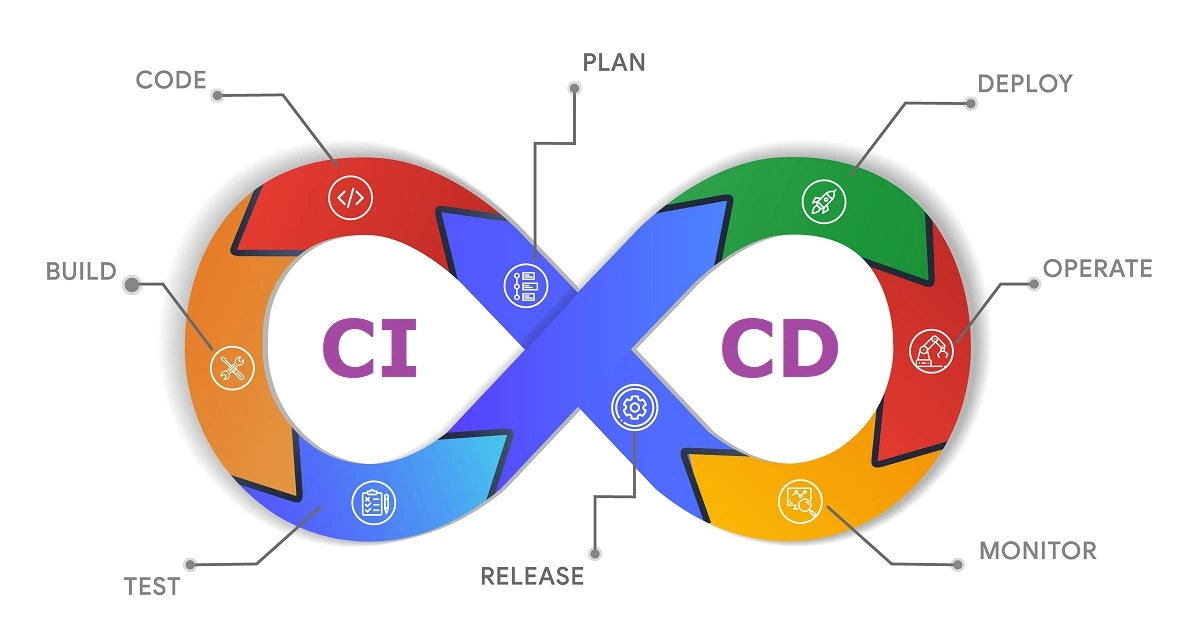
\includegraphics[width=1\textwidth]{figures/core/cicd.png}
\caption{Continuous Integration and Continuous Delivery~\cite{cicd}}
\label{fig:cicd}
\end{figure}

CI refers to the practice of frequently integrating code changes from multiple developers into a shared repository. The integrated code pieces are then automatically built and tested to ensure no conflict or issue emerges. This process ensures that the codebase remains stable and allows development teams to identify and fix issues early on. CI promotes collaboration, reduces the risk of integration problems, and enables rapid feedback, enabling the delivery of higher-quality software. 

CD extends the concept of CI by automating the software delivery aspects. Continuous Delivery enables safe, quick and sustainable shipment of changes into production. Those changes are typically new features, bug fixes, and configuration changes. CD relies on code that is always in a deployable state in order to make deployments as easy and straightforward to facilitate automation. Figure~\ref{fig:cicd} summarises the different steps of CI/CD.

CI/CD is closely linked to Agile methodologies. Both CI and CD foster the principles of frequent collaboration, iterative development, and continuous improvement. By automating repetitive and error-prone tasks, CI/CD enables teams to focus on delivering value, responding to changing requirements, and maintaining a sustainable pace. It aligns with Agile's emphasis on delivering working software quickly and adapting to feedback and evolving customer needs~\cite{fowler2006continuous,shahin2017continuous,duvall2007continuous,humble2010continuous}.

\subsection{Software Quality Assurance}
% Cite https://www.turing.com/blog/software-quality-assurance-and-its-importance/

Software development methodologies evolved throughout the years. In this context, one key aspect is also evolving accordingly: software quality. Users of any application have stronger expectations over time. They require not only bug-free products but also cheap, fast, secure, easy-to-use and respectful towards their privacy. For any business now, software quality is of utmost importance. It saves time and money, as repairing bugs or patching security issues too late can be very costly, it ensures competitiveness in the market and is also key to maintaining a good brand reputation among customers. This is when the role of Software Quality Assurance comes into place~\cite{galin2004software,beizer1984software,tripathy2011software}.

Software Quality Assurance (SQA) represents any set of methods, processes and activities applied during the life cycle of a software project to guarantee its quality, reduce and prevent defects during its development and confirm its alignment with the defined requirements. SQA is defined by many standards and norms across the industry, but several principles prevail:
\begin{itemize}[label={}]
    \item \textbf{Prevention}: The cost of software bugs is known to grow exponentially the longer it takes to be fixed. It is then important to allocate the necessary efforts to identify potential issues early in the development life cycle and to reduce the risk of shipping faulty products.  
    \item \textbf{Continuous improvement}: SQA is not a one-time check. It is a continuous process that needs to be followed at all times. It is also often required to adapt methodologies and processes in parallel with the evolution of the software especially at scale.
    \item \textbf{Stakeholder involvement}: To achieve good quality assurance, every stakeholder needs to be involved in the process, this includes managers, developers, testers, but also the customers or users. Good communication between all parties facilitates quick feedback and enables fast reactions.
    \item \textbf{Risk prioritisation}: SQA involves identifying and managing risks that could impact the quality of the software and taking proactive steps to mitigate them.
\end{itemize}

According to these principles, SQA activities are then defined and followed in a continuous manner.
\begin{itemize}[label={}]
    \item \textbf{Planning}: The first activity should be to clearly define quality standards that the end product should meet. This includes specifications, acceptance criteria and performance metrics. These blueprints should also indicate who is responsible for each task.
    \item \textbf{Reviews}: Through the iterations of the software development life cycle, reviews should be carried out to prevent software defects. This includes code reviews, writing documentation, and checking the requirements. If possible, this should be done by internal and external teams.
    \item \textbf{Testing}: SQA involves testing and validating the software. Performing multi-level testing is important to ensure better quality. This includes unit tests, integration tests, system tests and acceptance tests.
    \item \textbf{Monitoring}: Measuring and monitoring coding activities is important to keep track of quality indicators. This can be done using code coverage, bug-tracking systems and testing tools.
\end{itemize}

This dissertation focuses towards the software testing aspect.

% Evolving into CI and rapid integration

\subsection{Software Testing}

\subsubsection{Principles}

Software testing is a crucial and necessary aspect of software development ensuring the quality, reliability, and functionality of software systems. It involves systematically checking and evaluating the software against predefined requirements to align with user needs and expectations. The primary goal of software testing is to find bugs, defects or errors as early as possible in the development life cycle. According to some studies~\cite{costBug}, the cost of fixing a bug is growing exponentially the later it is found in the different phases of development and can go up to 100 times more costly if identified in production. \\

There are several key principles that guide software testing:

% To change 
\begin{itemize}[label={}]
    \item \textbf{Exhaustiveness:} Testing aims to achieve a high level of coverage, ensuring that all relevant functionalities, scenarios, and input combinations are tested. While it may not be possible to test every single possibility, testing efforts should be comprehensive to minimize the risk of undiscovered defects.
    
    \item \textbf{Independence:} Testing should be conducted independently of the development process to ensure impartiality. Testers should have a clear understanding of the software's functionality but should maintain a separate perspective to identify potential issues or deviations from requirements.
    
    \item \textbf{Early Start:} Testing should commence as early as possible in the software development life cycle. By incorporating testing from the initial stages, defects can be identified and resolved quickly, reducing the potential impact on future development phases.

    \item \textbf{Reproducibility:} Tests should be reproducible, allowing defects to be isolated and fixed reliably. This principle ensures that identified issues can be accurately communicated and resolved by the development team.

    \item \textbf{Traceability:} Testing should be traceable, meaning that test cases are linked to requirements and documented in a structured manner. This enables effective tracking of the testing process and ensures coverage of specific requirements.

    \item \textbf{Continuous Improvement:} Testing should be viewed as an iterative and continuous process. It involves learning from past experiences, analyzing test results, and refining testing strategies to enhance efficiency and effectiveness over time. Continuous improvement is key to optimizing the testing process and delivering higher-quality software.
\end{itemize}

By adhering to these principles, software testing helps to identify defects, enhance software quality, and ensure that software systems meet user requirements and expectations. It plays a vital role in reducing risks, enhancing customer satisfaction, and enabling the successful deployment of reliable software products.

\subsubsection{Levels of testing}

Testing is usually performed at different levels of granularity. The main type of tests are listed below:

\begin{itemize}[label={}]
    \item \textbf{Unit testing} focuses on verifying the functionality of individual components or units of code. It is typically conducted by developers and aims to ensure that each unit behaves as intended. Mock objects or stubs may be used to isolate units for testing.

    \item \textbf{Integration testing} verifies the interactions between different modules or components when they are combined. It aims to identify defects that arise from the integration of various units and ensures the proper functioning of the software as a whole.

    \item \textbf{System testing} involves testing the complete and integrated system against the specified requirements. It verifies the system's compliance with functional and non-functional requirements, such as performance, security, and usability. System testing is typically performed by a dedicated testing team.
    
    \item \textbf{End-to-end (E2E) testing} validates the entire software system as a whole, ensuring that all components work together as expected. It simulates real-life user scenarios to identify any issues or defects that may arise from the interaction and integration between different parts of the system.
\end{itemize}

Figure~\ref{fig:pyramid} represents the pyramid of tests illustrating the various type of testing. The concept of the pyramid is used to describe metaphorically the need for smaller tests and fewer high-level tests to facilitate the development and QA team to create and maintain high-quality software. Smaller tests like unit and integration tests are typically fast and easy to automate and maintain. Higher-level tests like System tests and E2E tests tend to be larger, more brittle and require more resources to write and to run. This is why it is generally advised to follow this pyramid-shaped structure when writing tests and to avoid the cupcake or ice-cream cone structure in order to facilitate the maintainability and efficiency of software testing. This list is non-exhaustive and, depending on the projects, other types of tests could be represented, such as Graphical User Interface (GUI) tests, to test visual components in the case of graphical applications, API tests, testing the different API endpoints or even manual testing, which is usually conducted occasionally or systematically on the overall system~\cite{contan2018test}.

\begin{figure}[ht]
\centering
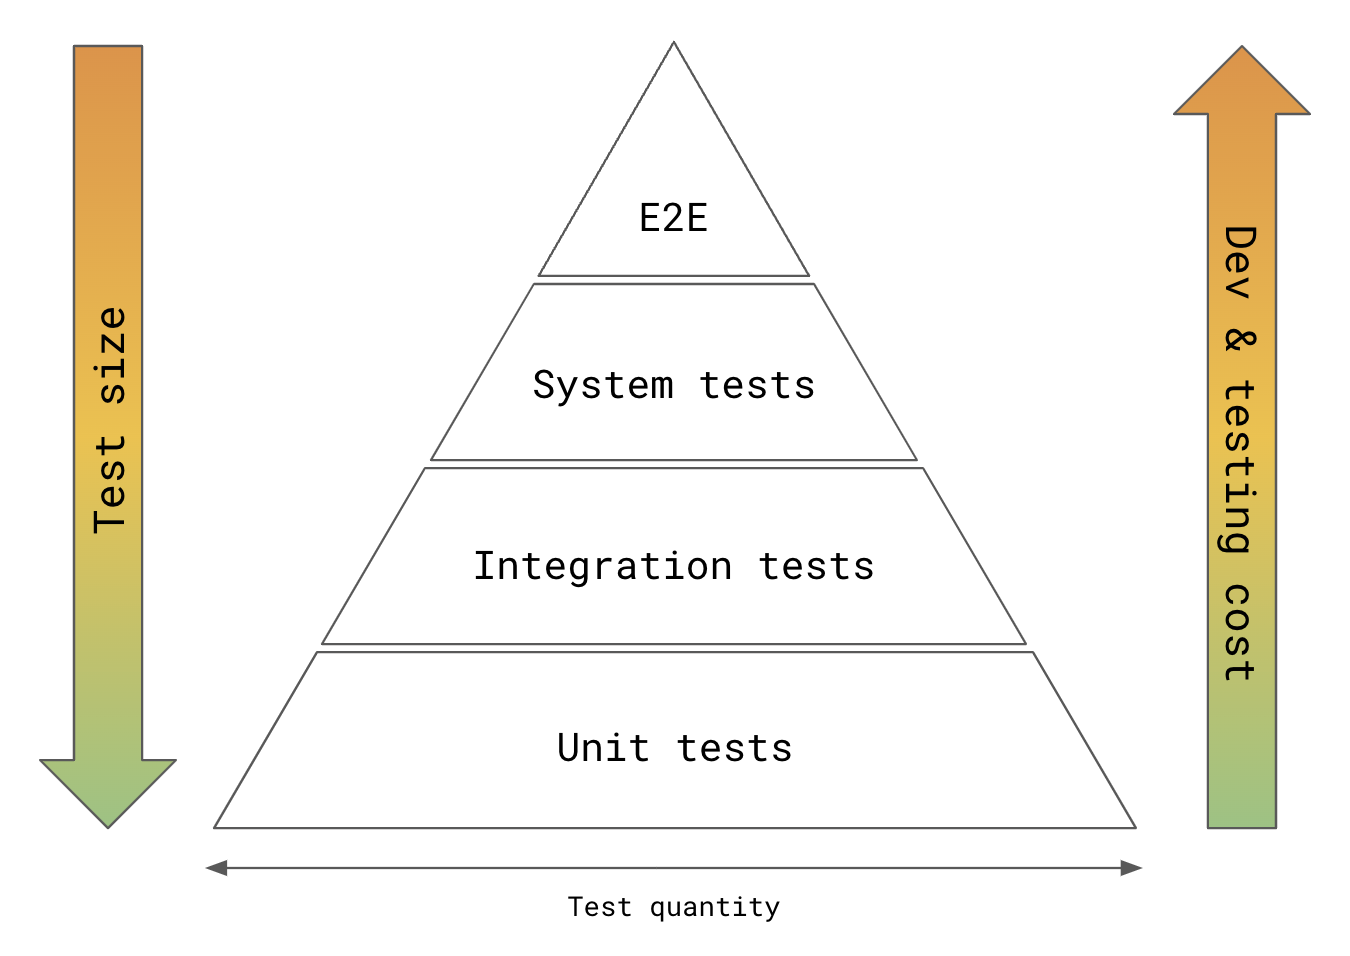
\includegraphics[width=0.8\textwidth]{figures/core/pyramid.png}
\caption{Pyramid of tests}
\label{fig:pyramid}
\end{figure}

\subsubsection{Test coverage}

One of the techniques used to assess the completeness of the testing process is test coverage. It is typically expressed as a percentage indicating the proportion of code or requirements covered by the tests. It can be measured at different test levels and can rely on different approaches, such as statement coverage, branch coverage or function coverage. Test coverage helps identify untested or under-tested areas of the software, enabling teams to focus their testing efforts and improve the overall quality of the system. However, it's important to note that achieving 100\% test coverage doesn't guarantee the absence of defects, as it's still possible to have undiscovered issues in the parts that are tested~\cite{malaiya2002software,malaiya1994relationship}.

\section{Challenges}

\subsection{Testing at Scale}

Challenges arise when software systems become large and complex over time. It is not surprising to find projects containing several hundreds of thousands of tests in big tech companies such as Google or Meta~\cite{Micco2017,Harman2018}. In such extreme contexts, where features are added at a very high rate (Google reports mention tens of thousands of commits per day~\cite{ivankovic2019code}) it becomes incredibly difficult to keep testing thoroughly as running all tests for every change would require too much time and resources. Even in optimal scenarios, final results can take several hours to compute before being sent for feedback to developers. \\

To alleviate issues linked with important time and computing resources required, several optimisation techniques can be leveraged:

\begin{itemize}[label={}]
    \item \textbf{Test parallelisation} relies on executing tests by dividing the test suite into smaller subsets and running them simultaneously in parallel test environments. Distributing test executions across multiple machines leveraging their combined resources can help expedite the testing process and reduce feedback time.
    
    \item \textbf{Commit batching} involves grouping multiple code changes into a single test run, thereby reducing the number of test executions and the overall testing time. Commit batching is a strategy that can help to find a good balance between timely feedback and testing efficiency, especially when dealing with large test suites and resource constraints environments. For example, if 10 commits are batched together and result in no test failure, then we have tested 10 commits with one execution thus saving nine executions. However, if a failure occurs it is not straightforward to know which build caused the failure. A bisection is then run to isolate the failing build. Further investigations to identify the culprit build and root cause remain challenging. Research works have been carried out to reduce the search space of bug-inducing commits ~\cite{batching, najafi2019bisecting, an2021reducing}.
    
    \item \textbf{Test Selection} is another technique that can be used to reduce the number of tests to execute. In this case, only the relevant tests are executed based on code changes or impacted areas. This reduces the number of tests run and speeds up the feedback cycle. This technique is commonly referred to as Regression Test Selection (RTS) and, even if it has been investigated for many years - several surveys date back to the 2000s~\cite{engstrom2010systematic,rothermel1996analyzing,graves2001empirical} - it remains a challenge to optimise test selection in CI~\cite{shi2019understanding} and to find efficient ways to select tests. 

    \item \textbf{Test Prioritisation} can also be leveraged to reduce testing costs and feedback time. Commonly referred to as Test Case Prioritisation (TCP), the idea consists of starting to test the critical tests or the ones having a strong ability to identify defects. Executing high-priority tests first helps to get rapid feedback. This approach ensures that important issues are identified early in the testing process. As an example, if only one test will fail for a given test suite execution, it is then better to have this test executed among the first ones.

\end{itemize}

\subsection{Automated Testing Research}

Many research directions are taken to help test more thoroughly software and to help with debugging tasks in a more automated and efficient way. The list below presents some of the main aspects drawing attention nowadays:

\begin{itemize}[label={}]
    \item \textbf{Mutation Testing} is a type of software testing used as a test adequacy criteria, \ie to assess the effectiveness and thoroughness of existing tests. It does so by introducing artificial faults, small syntactic changes, into the original program and then checking the ability of existing test suites to detect those changes. As we saw earlier, test coverage only cannot guarantee that a program is tested thoroughly. The challenge for mutation testing is that it can be computationally expensive and time-consuming, especially for large codebases. Many works try to reduce the number of mutants~\cite{Offut1993,siami2008sufficient} (\eg finding equivalent mutants), to identify and select relevant mutants~\cite{garg2022cerebro,ojdanic2022use,titcheu2020selecting} and to evaluate their applicability in the software evolution context~\cite{ojdanic2023MutantSelection,ma2020commit}.
    
    \item \textbf{Automated Test Generation} can reduce the effort and time required to create new test cases during the development process. Tools and frameworks exist to generate relevant test cases with regards to the targeted source code~\cite{fraser2011evosuite,fraser2012whole,pacheco2007randoop}. Different are commonly used for that purpose: code-based, property-based, random-based... One of the biggest challenge in automated test generation is linked with the test oracle problem: tools often face the challenge of determining the expected output or behavior of the system under test. Without a clear oracle, it becomes difficult to evaluate whether the generated tests are correct or not.
        
    \item \textbf{Fault Localisation} is a research area in software testing that focuses on identifying the specific locations of software defects. It aims to assist developers in quickly identifying the parts of the code that are responsible for the observed failures.
    Different approaches exist~\cite{papadakis2015metallaxis}. Spectrum-based approaches leverage information from the program's execution trace or coverage data to pinpoint potential fault locations~\cite{wen2019historical,de2016spectrum}. These approaches compute suspiciousness scores for program elements (e.g., statements, branches) based on the difference between passing and failing executions. Search-based approaches formulate fault localization as an optimization problem and employ search algorithms to explore the space of possible fault locations~\cite{leitao2020search,}. Machine learning approaches use statistical analysis or machine learning models to identify faults~\cite{li2019deepfl}. They leverage various code and program characteristics, such as code metrics, static analysis results or historical data. Common challenges in automated fault localisation research include the accuracy of fault localization results, the scalability to handle large codebases or the generalizability across different software contexts.
        
    \item \textbf{Automated Program Repair} aims at automatically patching defects. Similarly to fault localisation, APR includes different approaches, like search-based repair, constraint-based repair or pattern-based repair. Challenges remain to evaluate patch correctness and quality, to have tools scaling with the size and complexity of the software system and to promote the adoption of such approaches in real-world context~\cite{goues2019automated,qi2014strength,motwani2018automated}.

\end{itemize}

\subsection{Test Flakiness}

Most, if not all, of the approaches presented above, rely on deterministic tests and execution: when a given input results in a program state, we expect the output to be reproducible with similar input. This is not always the case, and developers often face what they call \textit{flaky tests}. 
Flaky tests are tests that pass and fail for the same code under test. 

\begin{itemize}[label={}]
    \item \textbf{It complicates the debugging} 
    One of the most common actions taken to debug a test that fails is to rerun it. Unfortunately in the case of a flaky test, it might be difficult to reproduce the error. Developers would then understand that something is wrong without figuring out what. This augments the time and effort given to debug and solve flakiness~\cite{perscheid2017studying}.
    
    \item \textbf{It reduces developers trust} 
    Flakiness is not always under the control of developers. A test might be flaky because of external dependencies not available at the time of execution or because of infrastructure issues. In this case, developers would tend to ignore signals from their tests. This can lead to real bugs being disregarded and ultimately results in less quality in the software~\cite{Eck2019}.
    
    \item \textbf{It alters existing techniques} 
    Outside the direct challenges faced by developers, flakiness can also impact automated software techniques. As we saw earlier, many automated testing approaches can be implemented to reduce testing costs. The presence of flakiness brings noise altering the efficiency of those approaches~\cite{qin2021impact,Cordy2019}.

    \item \textbf{It critically affects the industry}
    Flakiness is reported to be one of the major software testing challenges encountered nowadays. Several reports from the industry highlight this~\cite{JiangHuawei,Harman2018,Mozilla,FlakinessSpotify,FlakinessGoogle,GTAC2016}. For instance, at Google, there are 150 million test executions per day, and almost 16\% of their 4.2 million test cases have some level of flakiness~\cite{Micco2017}. This entails enormous computational resources since 2-16\% of the company's testing budget is dedicated to rerunning flaky tests~\cite{GTAC2016}. Perhaps worse, over 80\% of observed transitions (false Failures or Passes) at Google workflow are caused by flaky tests \cite{LeongSPTM19}, indicating an important level of uncertainty in the test signal.

\end{itemize}

% Add conclusion
The next chapter will give more details about the origins of flakiness and some examples. 

\section{Scope of the Thesis}

This dissertation largely focuses on the use of machine learning techniques to predict different aspects of flakiness, such as if a test is flaky or not, which part of the code under test is causing the flakiness, or which category of flakiness a flaky test belongs to. It also intends to better understand and assess their usability and validity in real-world scenarios. The subjects used for the different studies are coming from the open-source community. It is also worth noting that the studies mainly focus on automated functional testing: unit tests, integration tests and GUI tests but do not specifically address higher-level tests such as system tests or even manual tests as there tend to be fewer of them in open-source software.

\section{Overview of the Contribution and Organization of the Dissertation}

This section presents the contributions of this dissertation to address the aforementioned challenges related to flakiness as well as the organization of this dissertation as illustrated by Figure~\ref{fig:structure}. 

\subsection{Contributions}

The contributions of this dissertation are the following:

\begin{itemize}
    \item \textbf{Chapter 4: A Qualitative Study on the Sources, Impacts, and Mitigation Strategies of Flaky Tests} We performed a grey literature review and interviewed 14 practitioners in order to have a better understanding of the challenges linked with flakiness in the industry. We explore three aspects: the sources of flakiness within the testing ecosystem, the impacts of flakiness and the measures adopted when addressing flakiness. Our analysis showed that, besides the tests and code, flakiness stems from interactions between the system components, the testing infrastructure, and external factors. We also highlighted the impact of flakiness on testing practices and product quality and showed that the adoption of guidelines together with a stable infrastructure are key measures in mitigating the problem. Furthermore, we also identified automation opportunities enabling future research works.\\ \\
    
    
    \item \textbf{Chapter 5: A Replication Study on the Usage of Code Vocabulary to Predict Flaky Tests} Recent research works explored the possibility of detecting flaky tests using supervised learning. However, to reach industrial adoption and practice, these techniques need to be replicated and evaluated extensively on multiple datasets, occasions and settings. In view of this, we perform a replication study of a recently proposed method that predicts flaky tests based on their code vocabulary. We thus replicate the original study on three different dimensions. First, we replicate the approach on the same subjects as in the original study but using a different evaluation methodology, \ie we adopt a time-sensitive selection of training and test sets to better reflect the envisioned use case. Second, we consolidate the findings of the original study by checking the generalisability of the results for a different programming language. Finally, we propose an extension to the original approach by experimenting with different features extracted from the code under test.\\
    
    \item \textbf{Chapter 6: Predicting Flaky Tests Categories using Few-Shot Learning} While promising, existing flakiness detection approaches mainly focus on classifying tests as flaky or not and, even when high performances are reported, it remains challenging to understand the cause of flakiness. This part is crucial for researchers and developers that aim to fix it. To help with the comprehension of a given flaky test, this chapter introduces FlakyCat, the first approach to classify flaky tests based on their root cause category. FlakyCat relies on CodeBERT for code representation and leverages Siamese networks to train a multi-class classifier. We train and evaluate FlakyCat on a set of 451 flaky tests collected from open-source Java projects. Our evaluation shows that FlakyCat categorises flaky tests accurately, with an F1 score of 73\%. We also investigate the performance of FlakyCat for each category. In addition, to facilitate the comprehension of FlakyCat's prediction, we present a new technique for CodeBERT-based model interpretability that highlights code statements influencing the categorization.\\
    
    \item \textbf{Chapter 7: Pinpointing Classes Responsible for Test Flakiness} To mitigate the effects of flakiness, both researchers and industrial experts proposed strategies and tools to detect and isolate flaky tests. However, flaky tests are rarely fixed as developers struggle to localise and understand their causes. Additionally, developers working with large codebases often need to know the sources of nondeterminism to preserve code quality, \ie avoid introducing technical debt linked with non-deterministic behaviour, and avoid introducing new flaky tests. To aid with these tasks, we propose re-targeting Fault Localisation techniques to the flaky component localisation problem, \ie pinpointing program classes that cause the non-deterministic behaviour of flaky tests. In particular, we employ Spectrum-Based Fault Localisation (SBFL), a coverage-based fault localisation technique commonly adopted for its simplicity and effectiveness. We also utilise other data sources, such as change history and static code metrics, to further improve the localisation. Our results show that augmenting SBFL with change and code metrics ranks flaky classes in the top-1 and top-5 suggestions, in 26\% and 47\% of the cases. Overall, we successfully reduced the average number of classes inspected to locate the first flaky class to 19\% of the total number of classes covered by flaky tests. Our results also show that localisation methods are effective in major flakiness categories, such as concurrency and asynchronous waits, indicating their general ability to identify flaky components.\\
    
    \item \textbf{Chapter 8: The Importance of Discerning Flaky from Fault-triggering Test Failures} While promising, the actual utility of the methods predicting flaky tests remains unclear since they have not been evaluated within a continuous integration (CI) process. In particular, it remains unclear what is the impact of missed faults, \ie the consideration of fault-triggering test failures as flaky, at different CI cycles. In this chapter, we apply state-of-the-art flakiness prediction methods at the Chromium CI and check their performance. Perhaps surprisingly, we find that the application of such methods leads to numerous faults missed, which is approximately \nicefrac{3}{4} of all regression faults. To explain this result, we analyse the fault-triggering failures and find that flaky tests have a strong fault-revealing capability, \ie they reveal more than \nicefrac{1}{3} of all regression faults, indicating inevitable mistakes of methods that focus on identifying flaky tests, instead of flaky test failures. We also find that 56.2\% of fault-triggering failures, made by non-flaky tests, are misclassified as flaky. To deal with these issues, we build failure-focused prediction methods and optimize them by considering new features. Interestingly, we find that these methods perform better than the test-focused ones, with an MCC increasing from 0.20 to 0.42. Overall, our findings suggest that future research should focus on predicting flaky test failures instead of flaky tests (to reduce missed faults) and reveal the need for adopting more thorough experimental methodologies when evaluating flakiness prediction methods (to better reflect the actual practice).
\end{itemize}

\begin{figure}[ht]
\centering
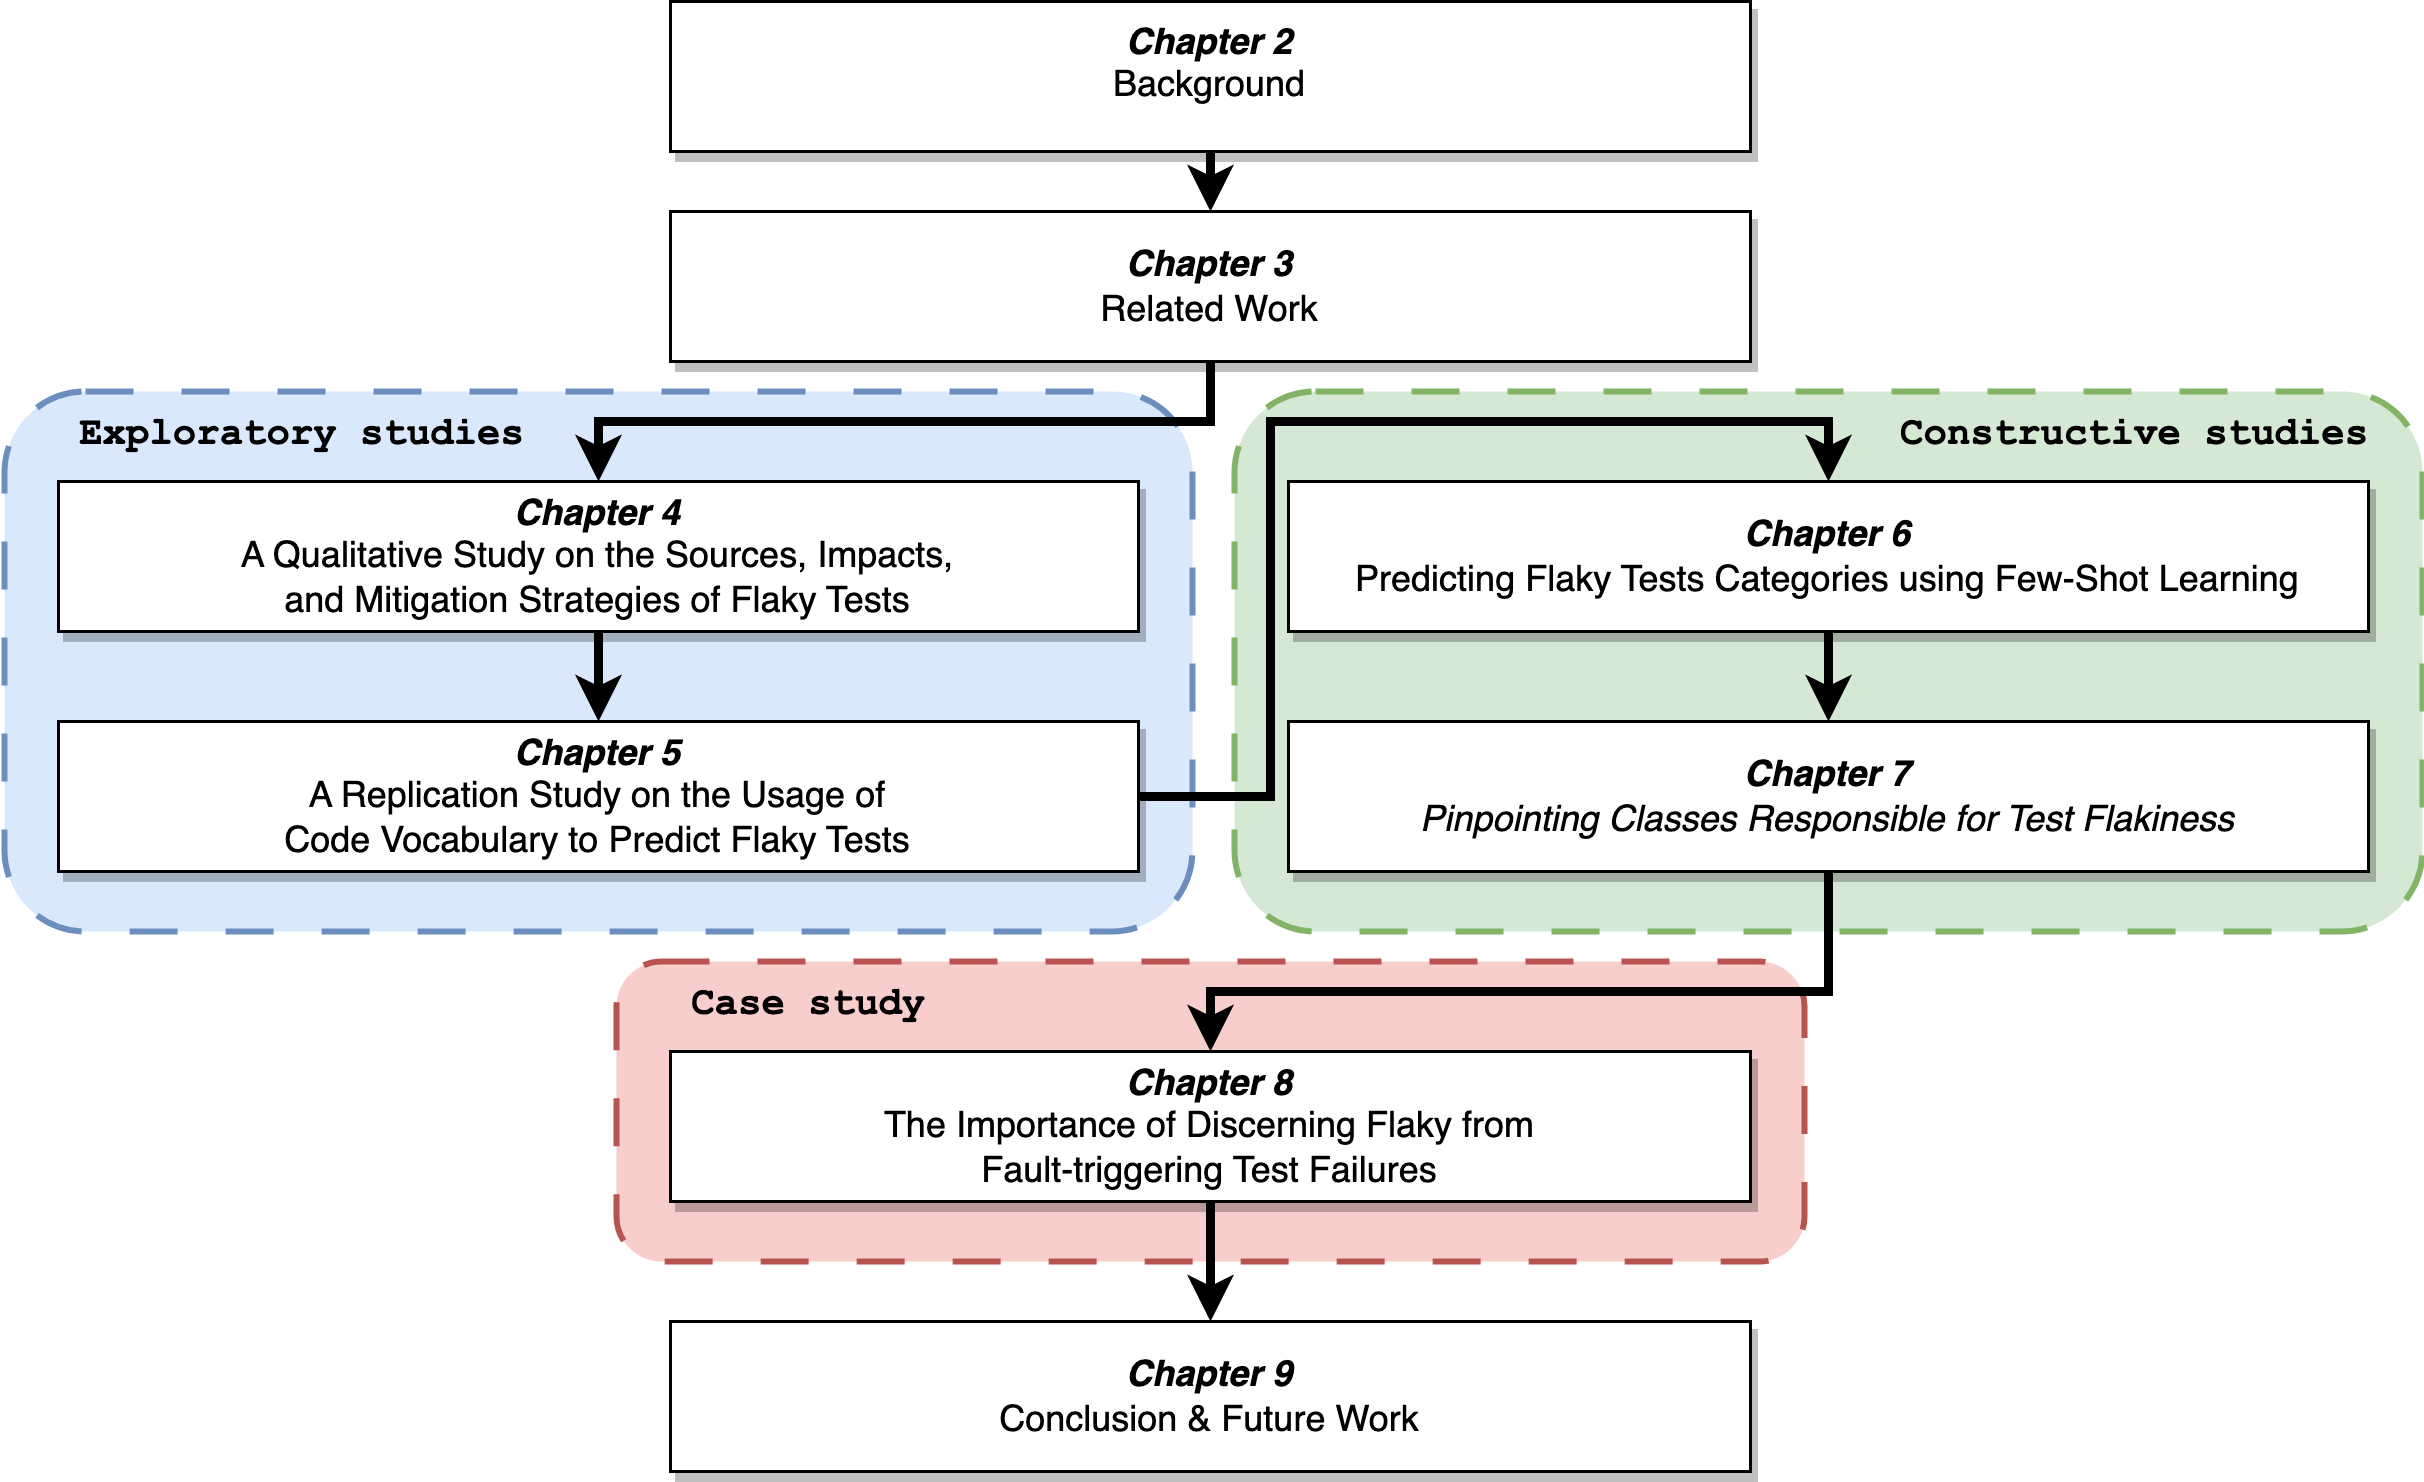
\includegraphics[width=1\textwidth]{figures/core/structure.png}
\caption{Structure of this thesis.}
\label{fig:structure}
\end{figure}

\subsection{Organization of the Dissertation}

In the remainder of this dissertation, Chapter 2 presents the technical background useful for a good understanding of this thesis. Chapter 3 discusses the existing works related to the contributions of this dissertation. Chapters 4 and 5 both contribute to the exploratory studies. The former presents a qualitative study on the sources, impacts and mitigation strategies of flakiness, and the latter details a replication study on the usage of code vocabulary to predict flaky tests. Chapters 6 and 7 are constructive studies. Chapter 6 presents FlakyCat, the first approach to classify flaky tests according to their category of flakiness and Chapter 7 introduces an approach to identify classes responsible for test flakiness. Chapter 8 is the last contribution of this dissertation. We present the case study of Chromium's continuous integration and highlight the importance of discerning flaky from fault-triggering test failures. Finally, Chapter 9 concludes the dissertation and presents future research directions.
